% id: 60-15
% book: 베이직쎈 확률과 통계 · 03 확률의 뜻과 활용
% section: 실전 감각 UP
% figure: tikz:fig-60-15
% answer: 
% answer_source: 
% variant_level: 0 (원본 전사)
% 이 파일은 build.mjs 가 items.json 에서 만든다. 고칠 때는 items.json 을 고친다.
\smash{\raisebox{1.5mm}{\dmkichul{베이직쎈 확률과 통계 60쪽 15번 · 서답형 · 서술형}}}
\noindent\begin{minipage}[t]{0.58\linewidth}\vspace{0pt}\raggedright 오른쪽 그림과 같이 평행한 두 직선 $l$, $m$ 위에 점이 각각 5개, 2개가 있다. 이 중에서 임의로 3개의 점을 택하여 선분으로 연결할 때, 삼각형이 만들어질 확률을 구하시오.\end{minipage}\hfill\begin{minipage}[t]{0.4\linewidth}\vspace{0pt}\centering \resizebox{\ifdim\width>\linewidth\linewidth\else\width\fi}{!}{% 60-15(인쇄 60쪽) — 평행한 두 직선 l, m 과 그 위의 점 5개·2개. 스캔 그림을 TikZ 로 다시 그림.
% 점에는 원문처럼 이름을 붙이지 않고, 라벨은 직선 이름 l·m 둘뿐이다(삼각형 개수 등 답의 근거는 적지 않는다).
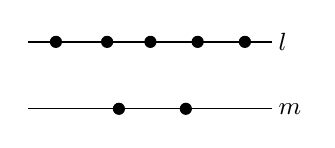
\begin{tikzpicture}[line width=0.5pt]
  \draw (0,0.85) -- (3.1,0.85);
  \foreach \x in {0.35,1.0,1.55,2.15,2.75} \fill (\x,0.85) circle (2.2pt);
  \node[anchor=west, inner sep=2pt, font=\small] at (3.1,0.85) {$l$};
  \draw (0,0) -- (3.1,0);
  \foreach \x in {1.15,2.0} \fill (\x,0) circle (2.2pt);
  \node[anchor=west, inner sep=2pt, font=\small] at (3.1,0) {$m$};
\end{tikzpicture}
}\end{minipage}\par
